% TeX source
%
% Author: Tetsuya Ishikawa <tiskw111@gmail.com>
% Date  : March 01, 2020
%%%%%%%%%%%%%%%%%%%%%%%%%%%%%%%%%%%%%%%%%%%%%%%%%%%%% SOURCE START %%%%%%%%%%%%%%%%%%%%%%%%%%%%%%%%%%%%%%%%%%%%%%%%%%%%%

本節ではカーネル法の概要を,数学的証明を用いずに説明してみたいと思う.
本節でカーネル法を説明する主な目的は,次節で行うRFFの解説において
事前に記号の理解を持って頂くことである.
厳密さが多少なりとも犠牲になるとについてはご容赦頂きたい.

やや深層学習に寄ったものの見方ではあるが,機械学習は主に
「データから特徴量を抽出する」ステップと「その特徴量を用いてタスクを行う」ステップに
大別される.図\ref{fig:kernel_method_and_feature_extraction}を参照されたい.
以下ではこの2つのステップを踏むことでカーネル法を概観してみよう.

\begin{figure}[t]
    \centerline{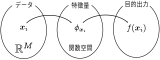
\includegraphics[width=200pt]{figures/kernel_method_and_feature_extraction.pdf}}
    \caption{カーネル法と特徴抽出}
    \label{fig:kernel_method_and_feature_extraction}
\end{figure}

\subsection{無限次元の特徴抽出と特徴関数}

入力データの集合を
$\mathcal{D} \triangleq \{ \bs{x}_i \in \mathbb{R}^{M} \bigm| i = 1, 2, \ldots, M \}$
とおく.
カーネル法は,入力データ$\bs{x}$から特徴量として関数,すなわち無限次元の特徴量を
抽出する手法である.このデータから無限次元の特徴量を抽出する関数,
ここれはそれを特徴関数と呼ぶこととするが,これを$\phi(\bs{x}, \bs{p})$で表すこととしよう.
具体例を挙げるとすれば,例えば
\begin{equation}
    \phi(\bs{x}, \bs{p}) \triangleq \exp \left( - \frac{\|\bs{x} - \bs{p}\|^2}{2 \sigma^2} \right),
    \label{eqn:feature_rbf}
\end{equation}
である.
これは有名なカーネル関数であるRFBカーネル (\textit{radial basis function kernel}) に対応する特徴関数である.
\begin{displayquote}\footnotesize\textsf{NOTE:}
後に説明するが,カーネル関数と特徴関数は\textgt{全くの別物}であるので注意されたい.
カーネル関数は特徴関数同士の内積として定義されるもので,特徴関数とは立場上全くの別物である.
ただ,RBFカーネルを含む有名どころのカーネル関数は結果として再生性をみたすゆえに
特徴関数とカーネル関数の関数形が一致し,説明する側としてはヤヤコシいのだが\ldots \verb|(^^;|
\end{displayquote}

注意して欲しいのは,特徴関数は入力データ$\bs{x}$を受け取り,$\bs{p}$に関する関数を返す関数である.
そういう意味で,特徴関数は$\phi(\bs{x}, \bs{p})$と書くよりも,$\phi_{\bs{x}}(\bs{p})$と書いた方が分かり良いであろう.
やや通常の関数表記から逸脱するが,以下では$\phi_{\bs{x}}(\bs{p})$の表記を用いることとする.
また,関数であることを特に強調したい場合は,引数の$\bs{p}$を省略して$\phi_{\bs{x}}$と書く.

\begin{displayquote}\footnotesize\textsf{NOTE:}
余談ではあるが,関数である$\phi_{\bs{x}}$を特徴「量」と呼称して良いものであろうか?
これはやや疑義を生ずる点であろうが,著者は量と呼称して問題ないと考えている.
関数は$L^2$空間に代表されるベクトル空間を構成する要素であるから,間違いなくベクトル「量」である.
\end{displayquote}

\subsection{特徴関数からのタスク実施}

さて,データ$\bs{x}$から特徴量$\phi_{\bs{x}}$が得られたところで,次はこの特徴量を用いて
回帰や分類などのタスクを行うことを考えていこう.
タスクの実施の仕方はタスクによって様々なのだが,最も一般的なアプローチは
\begin{equation}
    f(\bs{x}) = \idotsint_{\mathbb{R}^M} w(\bs{p}) \phi_{\bs{x}}(\bs{p}) \, 
    \mathrm{d}p_1 \cdots \mathrm{d}p_M,
    \label{eqn:task_kernel}
\end{equation}
という形で関数を構築する方法である.
回帰がしたいのであれば$f(\bs{x})$が目的の曲線を追従するように,
分類がしたいのであれば$f(\bs{x})$が対数尤度を出力するようにすれば良い.
ただし$w(\bs{p})$は学習パラメータに相当する関数である.
この関数を適切に学習させることで目的のタスクを実現するのがカーネル法である.

\begin{displayquote}\footnotesize\textsf{NOTE:}
式(\ref{eqn:task_kernel})が分かりづれぇ!と思ったそこの貴方.是非とも関数解析を習得されることをお薦めする.
式(\ref{eqn:task_kernel})はただの関数同士の「内積」であり,$f(\bs{x}) = \langle w, \phi_{\bs{x}} \rangle$と表記することもできる.
つまりやっていることは線形回帰と何も変わらず,ただ扱う空間がベクトル空間から関数空間に変わっただけのことである.
\end{displayquote}

もちろん,最適化パラメータが関数であるような最適化問題は数値計算問題として解きにくいので,
様々なテクニックを駆使してこれを有限次元の最適化問題に落し込み,その最適化を問題を解くことで学習を行うのである.

\begin{center}
メデタシ,メデタシ\ldots
\end{center}

\subsection{いやいや,カーネル関数はどこよ?}

え,カーネル関数はいつ出てくるのかって?
実はカーネル関数は,最適化問題をキチンと定式化し,その式をコネクリ回さないと出てこない.
本節ではその部分の理解にあまり体力を使いたくないので,先人が数式をコネクリ回した結果,以下が得られたということだけ指摘しておくに留めておく.
詳細については赤穂~\cite{Akaho2008}やBishop~\cite{Bishop2010}などを参照されたい.
\begin{enumerate}
    \item 関数$w$の最適化は有限次元のベクトルの最適化に落し込むことが出来る.ただしそのベクトルの次元は学習データ数$N$である.
          この関数の最適化問題を有限次元の最適化問題に落し込むテクニックは,カーネルトリックと呼ばれる.
    \item 上述1の最適化を解く上でも,最適化の結果を用いて推論を行う上でも,実は特徴関数$\phi_{\bs{x}}$は陽には出てこない.
          出てくるのは次の式
          \begin{equation}
              k(\bs{x}, \bs{y}) \triangleq \idotsint \phi_{\bs{x}}(\bs{p}) 
              \phi_{\bs{y}}(\bs{p}) \, \mathrm{d}p_1 \cdots \mathrm{d}p_M,
              \label{eqn:kernel}
          \end{equation}
          で与えられる関数$k$だけである.この関数$k$をカーネル関数と呼ぶ.
\end{enumerate}

さて,上記には2つの重要な事実が含まれている.
ひとつは,カーネルトリックによって関数次元の最適化問題を有限次元の最適化問題に落とし込めたとはいえ,
いまだに学習データ数$N$と同じだけの次元を持っているという点である.
これが本文書の冒頭で述べたカーネル法の弱点に直結しているのである.

もうひとつは,学習や推論を行う上で特徴関数は陽には出てこず,カーネル関数しか出てこないという点である.
ゆえに,一般的にはカーネル関数だけを設計し,特徴ベクトルには言及しない場合が多い.
ちなみに,式(\ref{eqn:feature_rbf})にて特徴関数の具体例をお見せしたが,これに対応するカーネル関数は
\begin{equation}
    k(\bs{x}, \bs{y}) = \exp(- \gamma \|\bs{x} - \bs{y}\|^2),
    \hspace{10pt} \gamma = - \frac{1}{4 \sigma^2},
    \label{eqn:kernel_rbf}
\end{equation}
である.これは式(\ref{eqn:kernel})を直接計算することで得られる.

さて,様々な式展開や証明を省略させて頂いたが,これでカーネル法のおさらいは終わりにして,早速RFFの定式化に移ろう.

\begin{displayquote}\footnotesize\textsf{NOTE:}
カーネル関数の説明が適当すぎないかって?
ご指摘の通りであるが,本文書としてはカーネル法の説明は前座にすぎないので,本節でパルプを3枚も4枚も費すことはしたくない.
もちろんカーネル関数がいきなり天から降ってくるのは本文書の想定読者を考えると論外である.
もっとスマートな導入の仕方があれば是非ご連絡頂きたい.
\end{displayquote}

%%%%%%%%%%%%%%%%%%%%%%%%%%%%%%%%%%%%%%%%%%%%%%%%%%%%% SOURCE FINISH %%%%%%%%%%%%%%%%%%%%%%%%%%%%%%%%%%%%%%%%%%%%%%%%%%%%
% vim: expandtab tabstop=4 shiftwidth=4 fdm=marker
